%% LaTeX Beamer presentation template (requires beamer package)
%% see http://latex-beamer.sourceforge.net/
%% idea contributed by H. Turgut Uyar
%% template based on a template by Till Tantau
%% this template is still evolving - it might differ in future releases!

% Voyager presentation for Warpstock Europe 2006
% Adrian Gschwend

\documentclass{beamer}
% Handout:
%\documentclass[handout]{beamer}

\mode<presentation>
{
\usetheme{Warsaw}
\setbeamercovered{transparent}
}

\usepackage{amsmath,amssymb}
\usepackage[latin1]{inputenc}
\usepackage{times}
\usepackage[T1]{fontenc}

\beamertemplatetransparentcovereddynamic

%\logo{
\includegraphics[height=0.5cm]{dws06.png}}

\title[netlabs.org - The Voyager Project]
{netlabs.org - The Voyager Project}

\subtitle
{A Workplace for the 21th Century}

\author[Adrian Gschwend]
{Adrian~Gschwend}

\institute[netlabs.org]
{
netlabs.org - Open Source Software for OS/2 and eCS
}

\date[17.11.2006]
{Warpstock Europe 2006, Cologne, Germany}

\subject{OS/2 and eCS development}
\keywords{OS/2 eCS eComStation}

% \AtBeginSubsection[]
% {
% \begin{frame}<beamer>
% \frametitle{Overview}
% \tableofcontents[part-1]
% \end{frame}
% }


\begin{document}

\begin{frame}
\titlepage
\end{frame}

\begin{frame}
\frametitle{Outline}
\tableofcontents[hideallsubsections]
\end{frame}

\section{History}

\begin{frame}
\begin{alertblock}{Warning}
This is not a very technical presentation!

(Please don't leave the room now ;-)
\end{alertblock}
\end{frame}

\subsection{Motivation}
\begin{frame}
\frametitle{One Year Ago}
After last years presentation:
\begin{itemize}
  \item<1-2>Joy
  \item<2>Shock
  \item<3->\textit{Why Voyager, my eComStation works just fine!?}
\end{itemize}
\end{frame}

\begin{frame}
\frametitle{Motivation, Hardware}
eCS and OS/2 works just fine \texttrademark
\begin{itemize}[<+->]
  \item Might be true nowadays
  \item Might be hidden for many users
  \item We (the developers) know the technical limitations
  \item Annoying kernel limitations and bugs
  \item Hardware envolves
\end{itemize}
\end{frame}

\begin{frame}
\frametitle{Motivation, Other Issues}
It's not just about the hardware\ldots
\begin{itemize}[<+->]
  \item The valuable stuff is done by the same few people
  \item Motivation is not what it used to be for various reasons
  \item It is annoying and frustrating to
  \begin{itemize}[<+->]
    \item write device drivers
    \item code around bugs
    \item port software and toolkits
    \item know that the work will be useless in a few years
  \end{itemize}
  \item Almost no new people are joining the community
\end{itemize}
\end{frame}

\begin{frame}
\frametitle{Conclusion}
\begin{block}{Conclusion}
If we do \textit{business as usual} it will not go on one day.
\end{block}
\end{frame}

\begin{frame}
\frametitle{Wouldn't it be nice?}
We can now either fall into depression or come up with some idea.

Why not
\begin{itemize}[<+->]
  \item rewrite what we like?
  \item profit from existing Open Source Software?
  \item \textit{do it right} ourself?
  \item start the whole idea on eComStation?
\end{itemize}
Thus the idea of Voyager was born!
\end{frame}

\subsection{The Journey}
\begin{frame}[allowframebreaks=0.6]
\frametitle{The Idea}
The Story so Far\ldots
\begin{itemize}
  \item Long process of thinking about the future for several years
  \item First idea with Kernel of MacOS X in Summer 2004
  \item First presentation of that idea at Developers Workshop 2005 in Dresden
  \item Reconsideration of this idea because it doesn't solve the main problem: Desktop
  \item New idea with OpenGL based Desktop with well known toolkits, developed at SYSTEMS fair in Munich
  \item Talks to various people and first presentation of that idea at
  Warpstock Europe 2005 in Dresden
  \item Presentation of first concept and design studies at Developers
  Workshop 2006 in Biel, Switzerland
  \item License decission during Summer 2006
  \item First 0.1 release of \textit{The Design of Voyager} released to the
  public for Warpstock Canada 2006
\end{itemize}
\end{frame}

\begin{frame}
\frametitle{What Voyager \textit{is not}}
\begin{itemize}
  \item Voyager is \textbf{not} the OS/2 and eCS killer!
  \item netlabs.org will \textbf{not} stop development for eCS software
  \item Voyager is not something you can use right now (yet)
  \item It is not vapoware
\end{itemize}
\end{frame}

\begin{frame}
\frametitle{The Goal}
There are many free desktop environments available, like KDE and GNOME. Our focus is different:
\begin{itemize}[<+->]
  \item SOM like object model, binary compatible (unlike everything else out
  there on Unix-like systems)
  \item Provide a WPS like desktop environment (\textit{OS/2 Feeling})
  \item Well integrated applications (drag \& drop, CUA, etc)
  \item Focus on localization right from the beginning (Unicode/UTF-8/16/32)
  \item Keep unique ideas like IOProcs and reimplement them
  \item Use as much existing code/apps as possible (as long as it makes sense),
  don't reinvent the wheel 
  \item Document what we do!
\end{itemize}
\end{frame}

\begin{frame}
\frametitle{Development Path}
\begin{itemize}[<+->]
  \item Development of Voyager should be possible on many platforms, starting on
  eCS
  \item Support for the most popular Unix-like systems is required
  \item eCS developers should be motivated to use SOM for new ideas because
  code can be partially reused
  \item Users can continue to use eCS as we know it today and still get new features
  \item Part-by-part replacement for smooth migration
\end{itemize}
\end{frame}

\begin{frame}
\frametitle{The Vision}
There is more to do\ldots
\begin{itemize}[<+->]
  \item A team of interested developers might start working on an OS/2 compatibility layer for Unix-like systems
  \item In long term we need a new kernel (discussion is open)
  \item Most of the OS/2 coders don't like the Linux design so other options are preferred
  \item If you can help out on that project, you are very welcome :)
  \item Final goal: our own distribution based on existing and new software
  \item And finally: \textit{Phase 3} (aka \textit{World Domination\texttrademark})
\end{itemize}
\end{frame}

\section{The Voyager Project}
\subsection{Introduction}
\begin{frame}
\frametitle{The Codename}
Why \textit{The Voyager Project}?
\begin{itemize}[<+->]
  \item Fits into OS/2 codenames (Star Trek)
  \item NASA Spacecraft: Probe since 1977, longest-lasting mission of NASA,
  visited Jupiter and Saturn and provided detailed images of them
  \item It is really just a codename, not a definitive name for a product.
\end{itemize}
\end{frame}

\subsection{Design of Voyager}
\begin{frame}
\frametitle{Voyager Components, now}
\begin{itemize}[<+->]
  \item Netlabs Object Model (SOM)
  \item Voyager Desktop (WPS)
  \item Cairo (GPI/GDI, what Peter loves ;)
  \item GTK+ (GUI Toolkit, PM)
  \item Triton (Multimedia Subsystem, MMPM/MMOS2)
\end{itemize}
\end{frame}

\begin{frame}
\frametitle{Voyager Components, next steps}
\begin{itemize}[<+->]
  \item Proper security concept
  \item Neptune (Window Manager for Cairo and Xlib)
  \item OpenGL based Cairo backend
  \item Xorg OpenGL device drivers (no Xlib necessary in mid-term)
\end{itemize}
\end{frame}

\section{Voyager Components}
\subsection{Under Development}

\begin{frame}
\frametitle{Netlabs Object Model}
\begin{itemize}[<+->]
  \item SOM is a binary compatible object model, no need to recompile objects (unlike on GNOME for example)
  \item There are some design documents from IBM itself (published in ACM)
  \item There is quite some documentation available written by former IBM employees
  \item Chris Wohlgemuth started to reimplement the concepts under the name NOM
  \item This is the base for a WPS like desktop
  \item Chris: Status? :-)
\end{itemize}
\end{frame}

\begin{frame}
\frametitle{NOM Design}
Rather complex design ;-)
FIXME
\end{frame}

\begin{frame}
\frametitle{Voyager Desktop}
\begin{itemize}[<+->]
  \item FIXME
\end{itemize}
\end{frame}

\begin{frame}
\frametitle{Cairo}
\begin{itemize}[<+->]
  \item modern, open source, cross-platform 2D API
  \item PDF/PS-like 2D API (hint: MacOS X Quartz)
  \item multiple output systems (screen, printer)
  \item OS/2 port exists, not accelerated so far
  \item OpenGL based backend exists, called Glitz (hint: MacOS X Quartz :)
\end{itemize}
\end{frame}

\begin{frame}
\frametitle{GTK+ Toolkit}
\begin{itemize}[<+->]
  \item Most used toolkit on Unix-like systems nowadays
  \item LGPL license (binary linking possible, unlike qt)
  \item Abstraction layer called GLIB
  \item Ongoing development
  \item wxWidgets and SWT are implemented on top of it
  \item Not yet available on eCS, PM port is evaluated right now
\end{itemize}
\end{frame}

\begin{frame}
\frametitle{Triton}
The OS/2 way to abstract codecs and such stuff is quite unique
\begin{itemize}[<+->]
	\item FIXME
\end{itemize}
\end{frame}

\subsection{Next Steps}

\begin{frame}
\frametitle{Neptune Window Manager}
A WM has to take care of
\begin{itemize}[<+->]
  \item the open client windows
  \item the client stacking order
  \item the client to virtual desktop assignment
  \item the session
  \item multiple screens
  \item client decorations
  \item ...
\end{itemize}
Status: Prototype done, developer is very busy with other things. Sourcecode
of prototype available soon.
\end{frame}

\begin{frame}
\frametitle{OpenGL Backend}
\begin{itemize}[<+->]
  \item OpenGL is the standard nowadays, only MS is doing their own game mit DirectX
  \item OpenGL allows fancy stuff like blending and 3D effects, no fun on 2D Hardware
  \item powerful API
  \item MacOS X is using it as backend, Xorg Project is moving towards OpenGL as well
\end{itemize}
\end{frame}

\begin{frame}
\frametitle{Xorg OpenGL Design}
\begin{columns}
\column[T]{5cm}
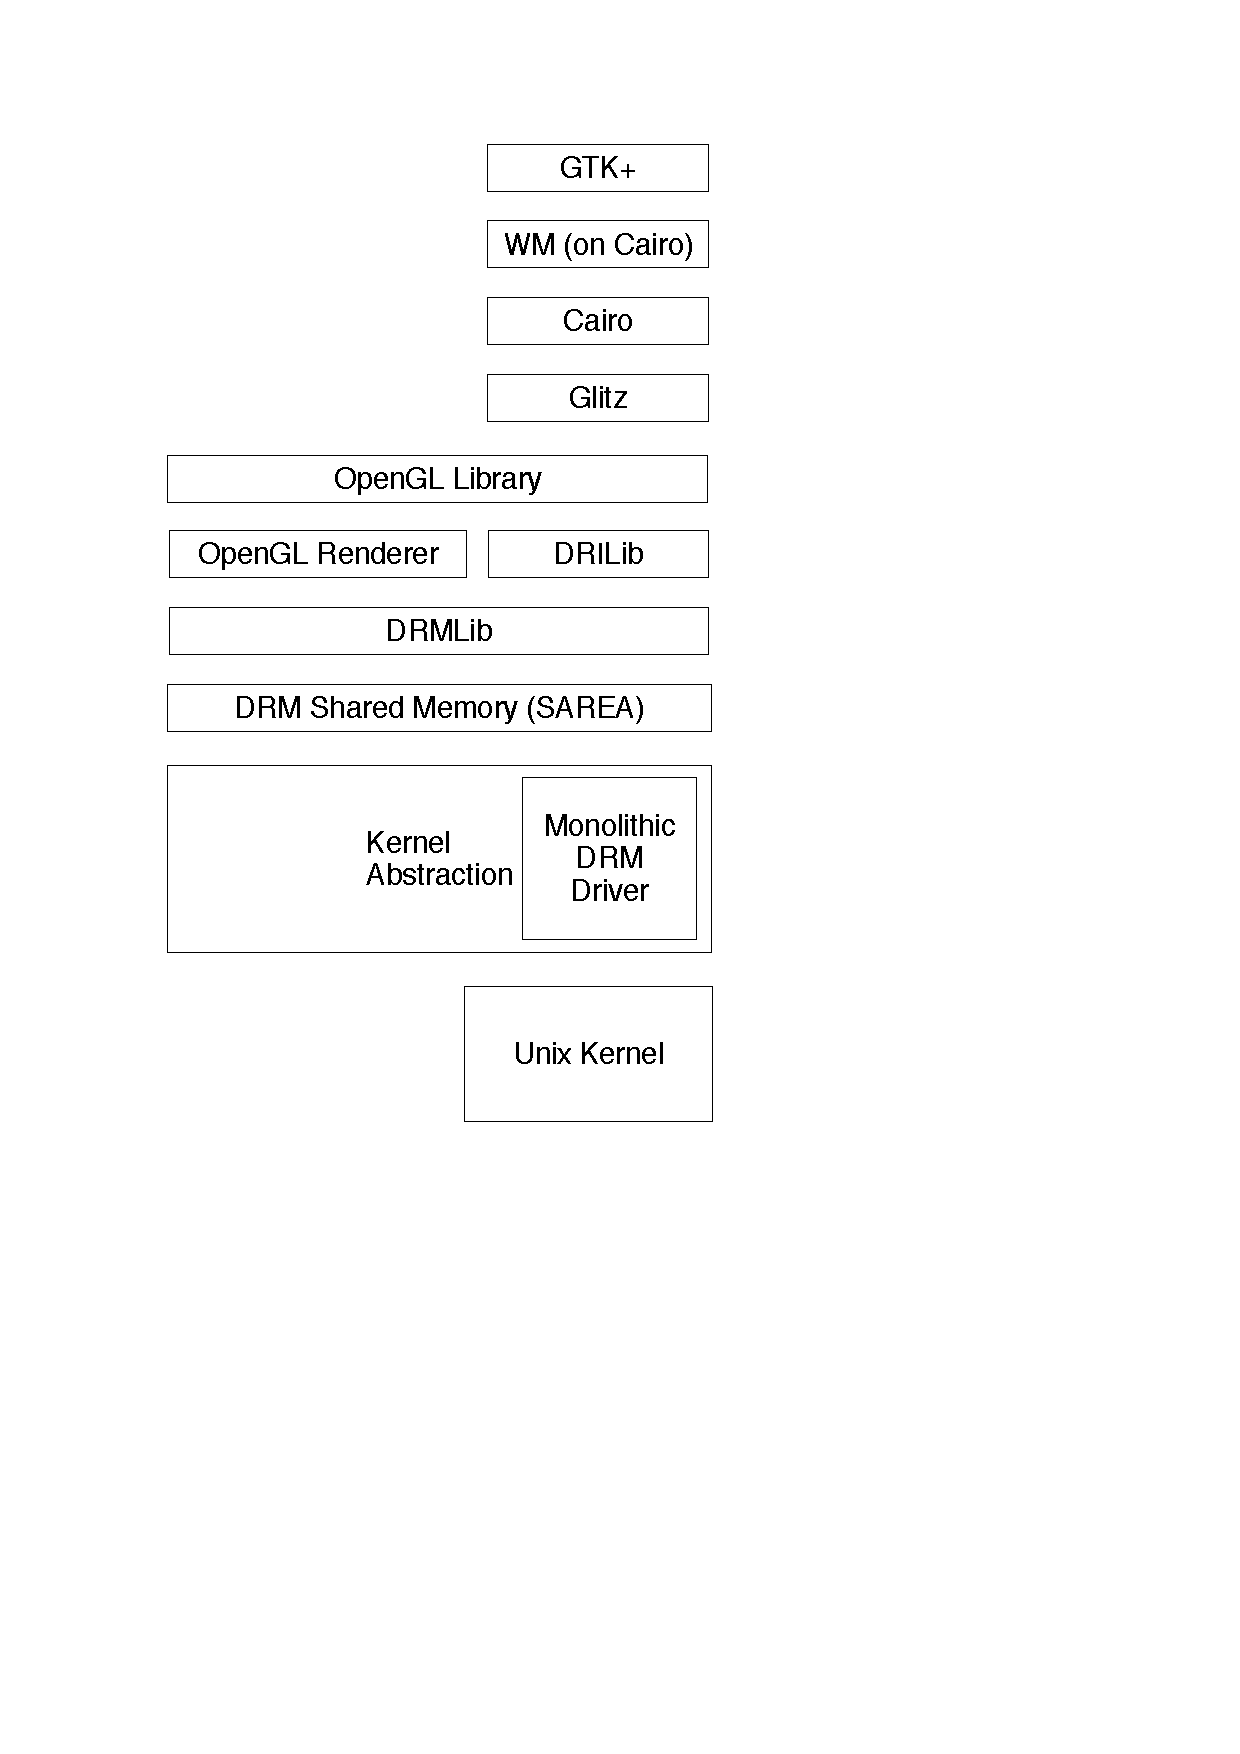
\includegraphics[width=3.5cm]{ogl-backend.pdf}
\column{5cm}
Simplified design of the Xorg OpenGL backend (taken from official docs), Xlib stripped out
\end{columns}
\end{frame}

\subsection{OS/2 and eCS Compatiblity}
\begin{frame}
\frametitle{Some Ideas}
People do ask for binary compatibility. We see the following options:
\begin{itemize}[<+->]
  \item Use a pure VM based solution - easy and will work well, already possible
  \item Rewrite the whole OS as proposed by some people - unrealistic, waste of ressources
  \item Implement a minimal OS/2 personality on top of an existing kernel and get binary compatibility to work
\end{itemize}
\end{frame}

\begin{frame}
\frametitle{OS/2 OS Personality}
To get a minimal OS/2 personality to work we would have to implement:
\begin{itemize}[<+->]
  \item \texttt{DOS*}, \texttt{MOU*}, \texttt{KBD*} and \texttt{VIO*} API's
  \item LX loader (Knuts kLoader)
  \item GRADD driver for OpenGL backend
  \item Some other things
\end{itemize}
Some things exist, like JdeBP - unfortunately not open source. Work on some
parts started, much work left.
\end{frame}

\begin{frame}
\frametitle{GRADD on OpenGL}
\begin{columns}
\column{3cm}
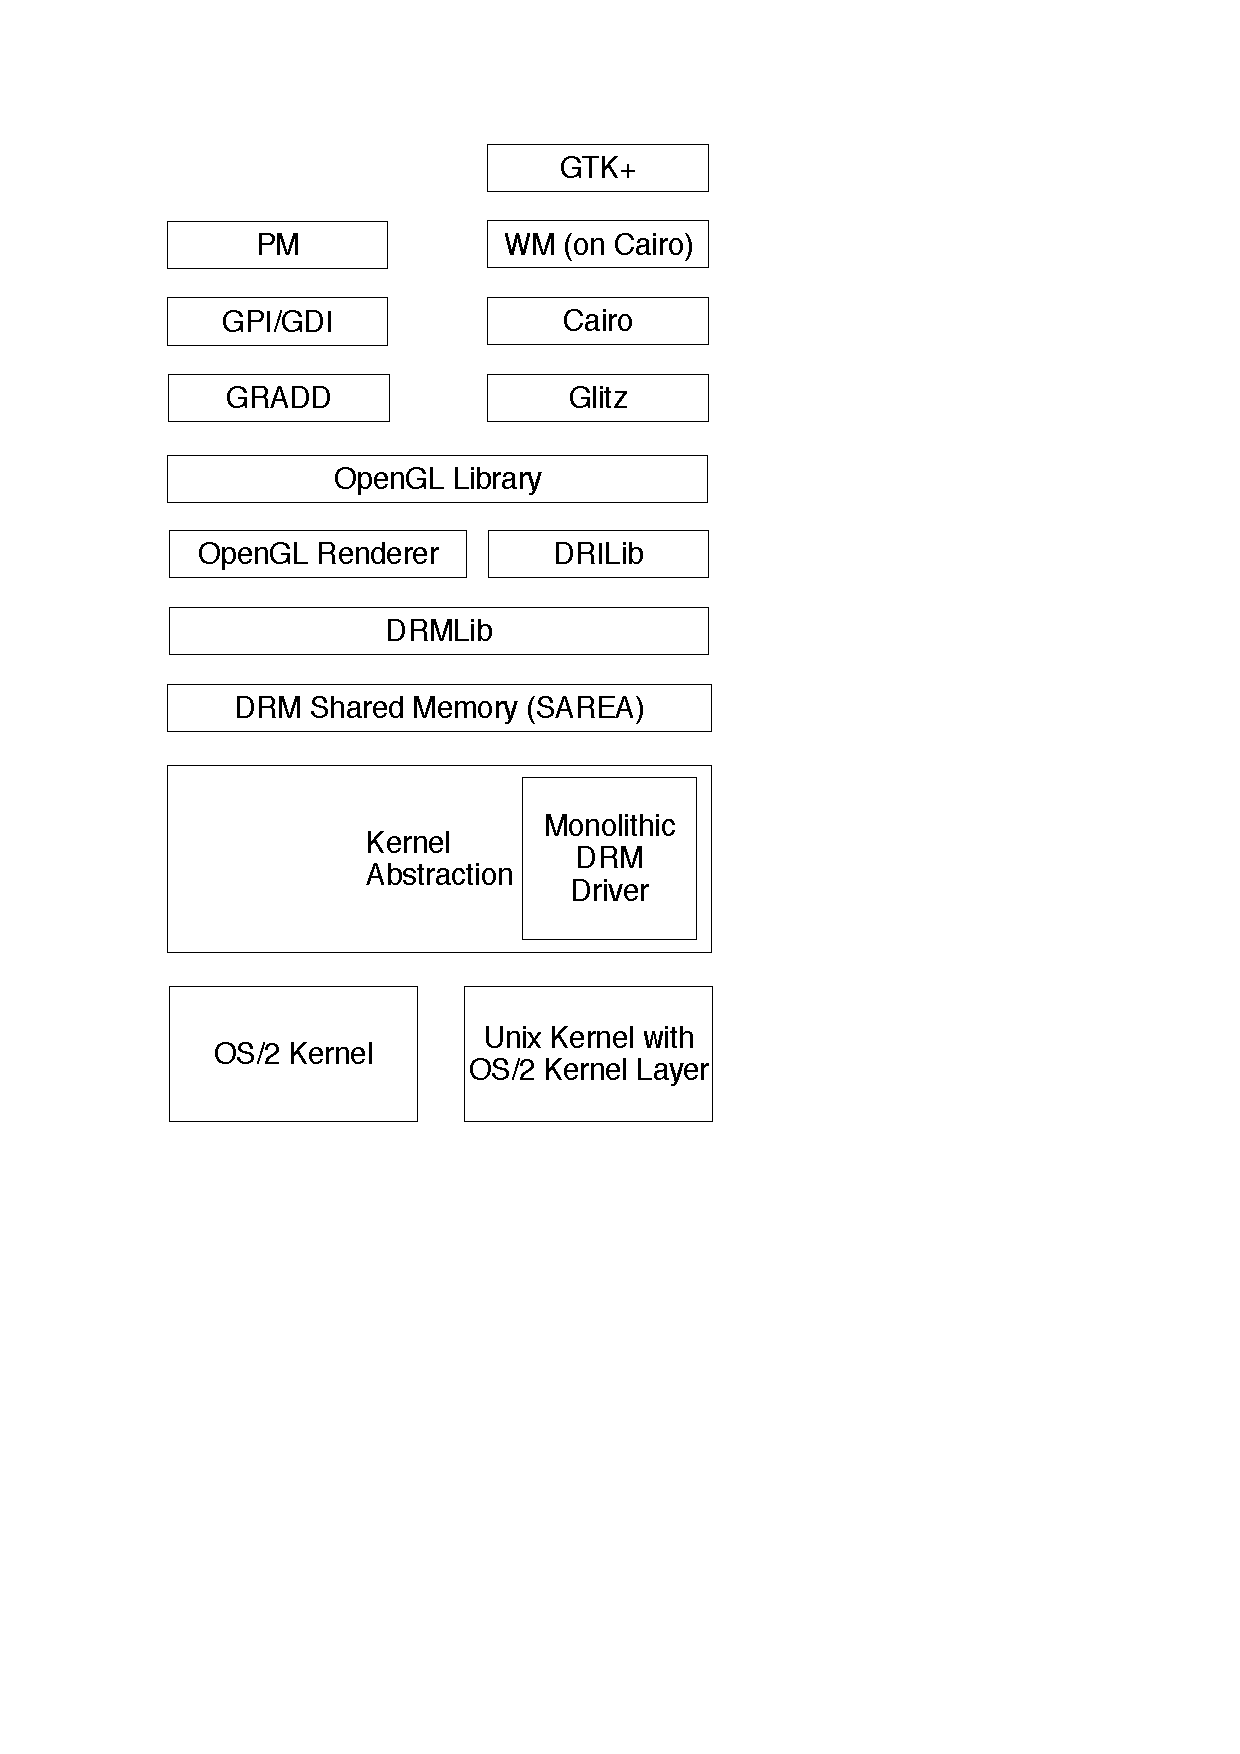
\includegraphics[scale=0.3]{ogl-gradd.pdf}
\column{6cm}
\begin{itemize}[<+->]
  \item OpenGL GRADD driver could be  used on OS/2 already, Xorg should work (with some effort)
  \item As soon as a OS/2 personality would work, one could migrate to the new
  kernel 
  \item This might become an important project for eCS anyway
\end{itemize}
\end{columns}
\end{frame}

\subsection{License}

\begin{frame}
\frametitle{Voyager License}
\begin{itemize}[<+->]
  \item we do not want to use GPL for our own code for various reasons
  \item the object model allows binary code, GPL would make that difficult
  \item we might use (L)GPLed code for parts when it makes sense to do that
  \item LGPL/CDDL dual license for Voyager core
  \item APL for sample applications
\end{itemize}
\end{frame}

\section{Roadmap}
\subsection{Work in Progress}

\begin{frame}
\frametitle{Timeline}
\begin{itemize}[<+->]
  \item First sourcecode is online!
  \begin{itemize}[<+->]
    \item Triton
    \item Netlabs Object Model
  \end{itemize}
  \item First version of \textit{The Design of Voyager} got released in October 2006
  \item New server for netlabs.org, new CMS with dedicated Voyager pages (work in progress)
  \item Goal: provide development environments for at least two platforms ASAP
\end{itemize}
\end{frame}

\begin{frame}
\frametitle{Join the Project}
\begin{itemize}[<+->]
  \item Go to \texttt{http://voyager.netlabs.org}
  \item Check the Voyager Wiki and FAQ
  \item Join the Voyager Mailinglist at
  \item join the \texttt{\#netlabs} IRC channel (see
  \texttt{http://www.ecomstation.com/chat.phtml}) 
  \item Contribute to \textit{The Design of Voyager}
  \item Contribute to NOM, Triton, compatibility layer etc.
  \item Translate as soon as first text is available
  \item Support us with money
\end{itemize}
\end{frame}

\begin{frame}
\frametitle{Voyager?}
We talked about what Voyager is not, so what is it then?
\begin{itemize}[<+->]
  \item It is a great motivation to go on with eCS
  \item It is a ambizioniertes FIXME project
  \item It is a great challenge
  \item It will become a great piece of software
  \item The first step to \textit{World Domination\texttrademark}
\end{itemize}
\end{frame}


\begin{frame}
\frametitle{Q\&A}
	Questions?
\end{frame}

% \begin{frame}
% \frametitle{About this Presentation}
% This presentation was done using the \LaTeX beamer class
% (\texttt{http://latex-beamer.sourceforge.net}). \texttt{pdflatex} was used to
% convert it to a PDF file.
% 
% \LaTeX source of the file is available in the Voyager Subversion repository at
% \texttt{http://svn.netlabs.org/v_doc}
% \end{frame}

\end{document}
